\documentclass[12pt, a4paper]{article}
\usepackage{blindtext, titlesec, amsthm, thmtools, amsmath, amsfonts, scalerel, amssymb, graphicx, titlesec, xcolor, multicol, hyperref}
\usepackage[utf8]{inputenc}
\hypersetup{colorlinks,linkcolor={red!40!black},citecolor={blue!50!black},urlcolor={blue!80!black}}
\newtheorem{theorem}{Theorema}[subsection]
\newtheorem{lemma}[theorem]{Lemma}
\newtheorem{corollary}[theorem]{Corollarium}
\newtheorem{hypothesis}{Coniectura}
\theoremstyle{definition}
\newtheorem{definition}{Definitio}[section]
\theoremstyle{remark}
\newtheorem{remark}{Observatio}[section]
\newtheorem{example}{Exampli Gratia}[section]
\newcommand{\bb}[1]{\mathbb{#1}}
\renewcommand\qedsymbol{Q.E.D.}
\title{title}
\author{Harry}
\date{\today}
\begin{document}
\maketitle
%\tableofcontents
\begin{figure}[htbp]
	\centering
	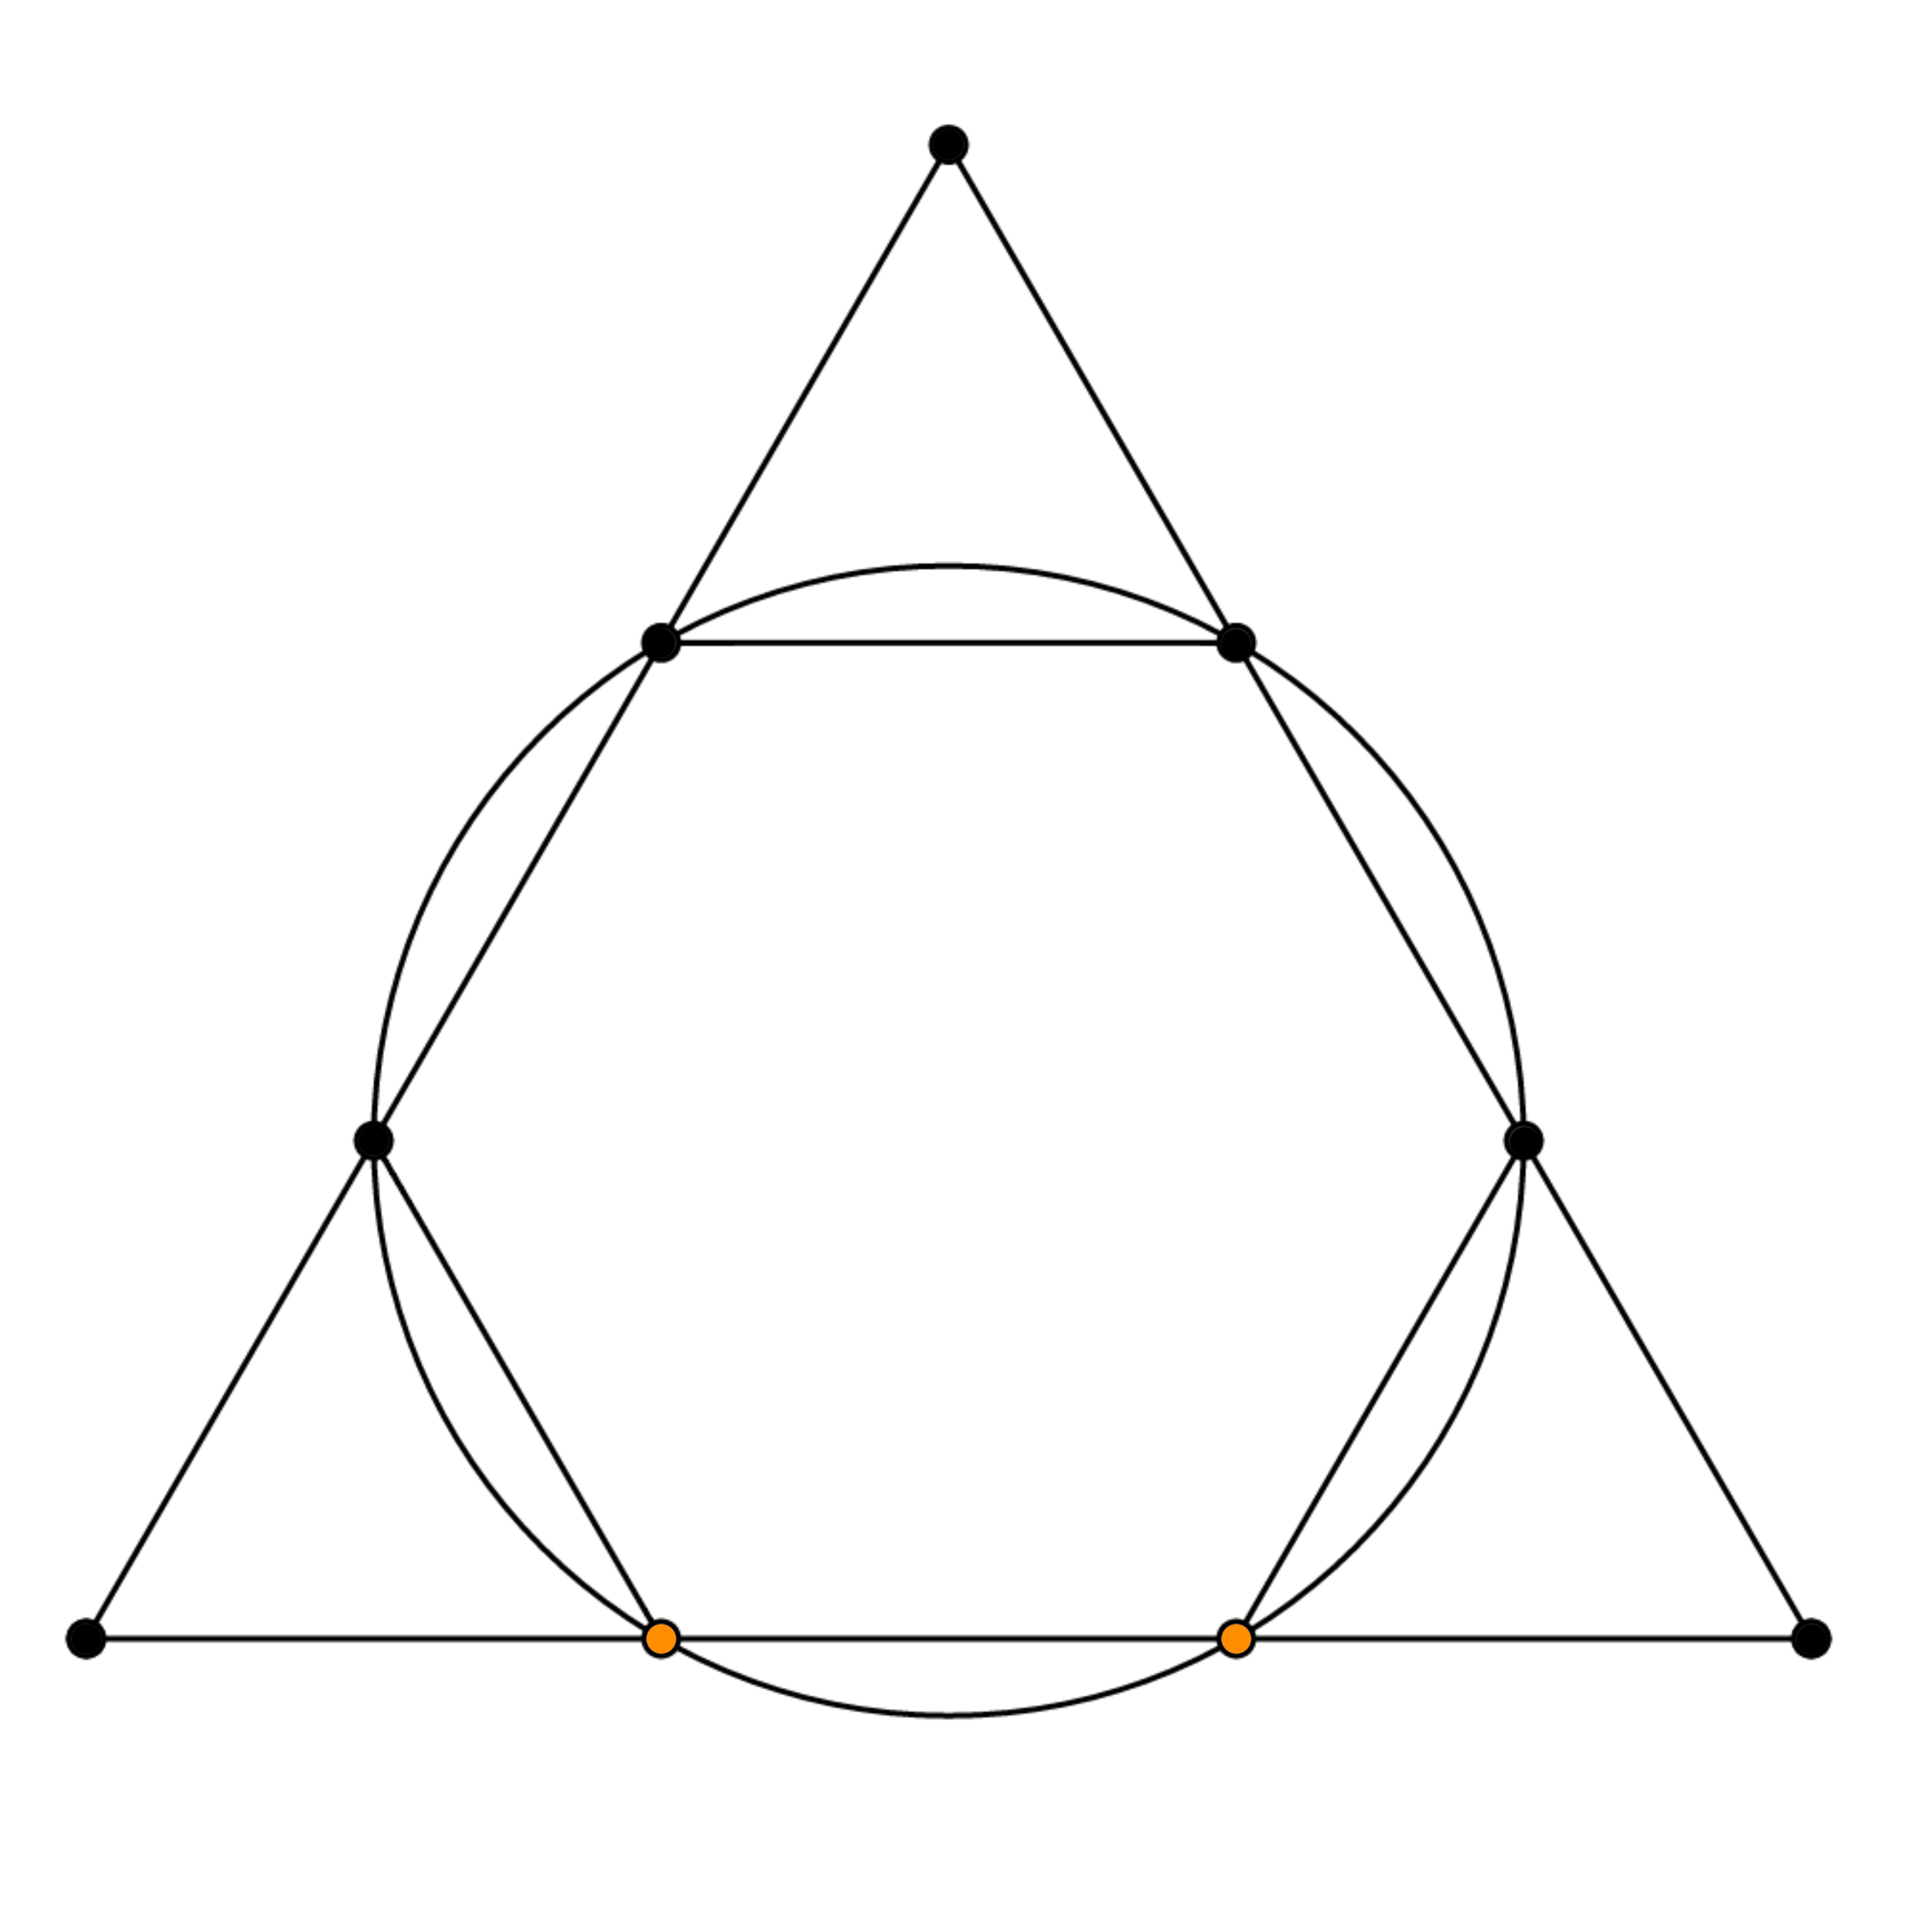
\includegraphics[width=0.8\textwidth]{./figure-1.png}
	\caption{Caption}
	\label{fig:Caption}
\end{figure}

% law of cosines 

\begin{theorem}
	\label{thm:1}
	Let $a, b, c$ be the sides of a triangle. Then 
	\begin{equation}
		c^2 = a^2 + b^2 - 2ab\cos\theta
	\end{equation}
\end{theorem}



\end{document}

